\documentclass[a4paper, 12pt]{article}
\usepackage{sbc-template}

\usepackage{graphicx}
\usepackage[brazil]{babel}
\usepackage[utf8]{inputenc}
\usepackage{epsfig}
\usepackage{float}
\usepackage{graphics}
\usepackage{url}
\usepackage[tight,footnotesize]{subfigure}
\usepackage{stfloats}
\usepackage{enumerate}
% \usepackage[left=3cm,top=3cm,right=3cm,bottom=3cm]{geometry}


% correct bad hyphenation here
\hyphenation{op-tical net-works semi-conduc-tor}


\begin{document}

\title{Arquitetura para Mitigação de Ataques DDoS}

\author{
Cinara Menegazzo\inst{1},
Fernando Cezar Bernardelli\inst{1}, \\
Fernando Henrique Gielow\inst{1},
Nadine Lipa Pari\inst{1}
}
   

   
\address{Departamento de Informática -- Universidade Federal do Paraná\\
  Caixa Postal 19.081 -- 81.531-980 -- Curitiba -- PR -- Brasil
  \email{\{cmenegazzo,fcb06,fhgielow,nelpari\}@inf.ufpr.br}
}     

\maketitle


% {
% \begin{center}
% {\LARGE \textbf{Arquitetura para Mitiga\c{c}\~{a}o de Ataques DDoS}}
% \vskip 0.5cm
% {\Large Cinara Menegazzo, Fernando Cezar Bernardelli, \\ Fernando Henrique Gielow, Nadine
% Lipa Pari}
% \end{center}
% }
\section*{\emph{Resumo}}
\emph{Aqui sera colocado o resumo deste trabalho}
A maioria das propostas para mitigar DDoS são de natureza reativa.

%\section{divisões do artigo}
% 2-trabalhos correlatos - sessão para revisar alguns mecanismos detecção e de mitigação de DDoS
%
%3- CLoud ou entra este tema direto na proxima sessao... 
%4 ou 3 se anterior nao existir - 
%
%Apresentação do servico e modelo de ataque (descrever o contexto da nossa proposta aqui entraria cloud e DDoS em cloud, qual a nosso modelo de ataque, composto por quantos zumbis etc...efeito do ataque, tipo de DDoS que usaremos...) que usaremos para mitigar, aqui entraria blacklist....
%
%Próxima seção descrever o esquema proposto para mitigar DDoS na cloud, nossa arquitetura e como funciona....e tempo requerido para parar um ataque ou detectar um.....aqui se levantaria metricas????
%
%Outra seção para descrever a experimentação(não gosto deste termo) da proposta-talvez análise de desempenho ou e  análise de resultados...modelo de experimentação, etc....
%Conclusao


\section{Introdução}


Diversas pesquisas e propostas têm sido desenvolvidas buscando soluções para problemas da Internet atual, que se propagam para a Internet do Futuro (IF). Tais problemas podem ser amplamente categorizados em nas áreas de mobilidade, qualidade de serviço e segurança, os quais ainda caminham para aceitáveis soluções.

Alguns paradigmas mudaram nestas últimas décadas. Hoje, tem-se os dados e aplicações disponibilizados em localizações físicas distintas e desconhecidas. Outra grande mudança ocorreu na forma de administrar um sistema, que antes era local com seus usuários e servidores característicos. Agora, tal sistema é hospedado em ambientes construídos pelo compartilhamento de recursos de diversos sistemas autônomos (AS) e heterogêneos.

O uso massivo dos recursos disponibilizados na Internet e toda a conectividade que este ambiente computacional proporciona, com serviços para uso pessoal, comercial ou acadêmico, torna este ambiente alvo fácil para códigos maliciosos, agravados pela forma como a arquitetura TCP/IP pode favorecer um atacante. O protocolo IP (\emph{Internet Protocol}) omite as informações da verdadeira identidade de um emissor, essa não autenticação da fonte permite ao atacante realizar o ataque contra a vítima, ainda permanecendo anônimo e impune.

Apesar de esforços de pesquisadores por muitos anos, um tipo de ataque que ainda representa sérias ameaças a muitos servidores na Internet é o ataque de DoS (\emph{Denial of Service}), configurando-se como um dos principais desafios de segurança que atualmente se propaga para a IF. 


A melhor forma de se defender deste tipo de ataque é a prevenção e a reação. O ataque por DoS não visa invadir um computador para obter informações confidenciais, nem tão pouco alterar informações armazenadas nele. Seu objetivo é a indisponibilizar um serviço que está sendo fornecido, utilizando-se do encaminhamento de grandes quantidades de tráfego ao hospedeiro do serviço, de forma que este não consiga responder a todas as requisições que lhe são encaminhadas. 

O problema se torna ainda mais crítico quando diversos geradores de tráfego distribuídos intensificam o encaminhamento de tráfego, caracterizando um ataque de DDoS \emph{Distributed Denial of Service} \cite{Sachdeva08ddosincidents}. O resultado obtido é o congelamento, a reinicialização, ou ainda o esgotamento completo de recursos necessários do hospedeiro. Os serviços que mais sofrem com este tipo de ataque são aqueles que permitem requisições anônimas como serviços web. Assim, o desafio de eliminar os ataques de DDoS está na dificuldade de determinar a diferença entre pacotes legítimos e pacotes de atacantes \cite{Li:2009:DDA:1683304.1684620}.


Com as novas arquiteturas de rede e de aplicações que configuram a IF, surgem sistemas complexos e robustos como \emph{clouds}, onde o desafio de mitigar ataques deste tipo torna-se ainda mais necessário.  O poder de
alocar recursos para suportar um ataque deste tipo em \emph{cloud}  agora torna-se
possível, porém crescem também os custos do usuário para manter tais recursos, o que
carateriza-se como eDDoS (\emph{economic Distributed Denial of Service}) \cite{Soon:10}.
  
A maioria das soluções comuns oferecidas para mitigar DDoS em \emph{cloud} se baseiam inteiramente na maior alocação de
recursos [referenciar???]. 
%
Algumas abordagens diferenciadas se mostram inadequadas por premissas que nem sempre são verdadeiras ou por serem custosas demais \cite{Bakshi:10}, \cite{Liu:2010:NFD:1866835.1866849}.
%,  colocar mais referencias...... 
Existem diversos registros de ataques que abalaram a Internet nos últimos tempos, como os ocorridos contra o Yahoo!, eBay, Amazon.com, e diversos outros \emph{sites} populares em fevereiro de 2000.  No início de 2011 se observou o ataque sofrido pelo hospedeiro de \emph{blogs}, WordPress, que enfrentou o pior ataque de DDoS de sua história \cite{infoexame}. Ataques deste tipo ainda estão por serem disparados em proporções alarmantes, confirmados por descobertas recentes da engenharia aplicada capaz de gerar redes de zumbis, como o caso da rede TDL-4 que é classificada por especialistas em segurança como “não perfeitamente, mas praticamente indestrutível”, com aproximadamente 4,5 milhões de infecções só em 2011 \cite{tdl4}. Portanto, a mitigação de DDoS em \emph{clouds} ainda demanda pesquisas.

O objetivo deste trabalho é elaborar uma arquitetura para mitigação de ataques de
DDoS executados sobre uma aplicação hospedada em uma \emph{cloud}. Esta
arquitetura deverá monitorar o tráfego da aplicação e, quando
detectar ocorrência de ataque de DDoS, será responsável por criar uma nova
instância desta aplicação, garantindo que nenhum tráfego malicioso a alcance. 

\textbf{CHANGEME},
Para que este trabalho possa ser.....este artigo está divido conforme 
Na primeira seção estão descritos a motivação e o objetivo deste trabalho, expondo o ambiente de problema e solução que será abordado pela pesquisa. NA seção dois, um levantamento dos trabalhos relacionados é descrito para que se posicione quanto as soluções já existentes. O cenário/arquitetura de .....na seção três

%
%Uma arquitetura de \emph{cloud} pode representar um ambiente propício a ataques por ser usado por diversas pessoas de diversas organizações com suas aplicações e sem o menor controle ou entendimento das configurações ou rede envolvida.
%
%Nos trabalhamos com o targeted attack????
%In a tar-
%geted attack, an adversary wants to gain a critical mass in a
%specific subnet, for example, to attack a specific application
%hosted in that subnet.




\section{Trabalhos Relacionados}

A necessidade de proteger ou mitigar as arquiteturas de rede de ataques de DDoS tem sido reconhecida tanto no meio acadêmico quanto comercial. Segundo \cite{1039856}, três são as linhas de defesa contra ataques de DDoS, compreendendo a prevenção, a reação, ou ambas, na chamada defesa híbrida. A prevenção tenta eliminar a possibilidade de ataques de DDoS evitando negação de serviço para os clientes legítimos, enquanto a reação detecta o ataque e responde imediatamente, a abordagem híbrida combina os métodos prevenindo e reagindo à ataques.

As pesquisas que envolvem propostas de mitigação para DDoS em arquiteturas de \emph{cloud}, ainda são consideradas incipientes e distantes de uma convergência. Dentre as poucas propostas para estes ambientes destaca-se o \emph{framework} pró-ativo CluB, criado por \cite{Hazelhurst:2008:SCU:1456659.1456671}, que considera uma \emph{cloud} como uma rede constituída de um conjunto de \emph{clusters}, ou \emph{Autonomous Systems} (AS) e sugere
que sejam selecionados determinados roteadores para análise de tráfego, dispostos de forma distribuída para evitar que as requisições maliciosas alcancem a aplicação. Estes roteadores ficam responsáveis por gerar \emph{tokens} de autenticação para legitimar os pacotes e a autenticação corresponde à entrada, saída ou trânsito na arquitetura. Cada \emph{cluster} tem seu código de autenticação e os códigos são trocados periodicamente, podendo ser gerados por uma função \emph{hash}, como MD5 ou SHA. O uso de ferramentas apropriadas de criptografia e atualizações periódicas de componentes da infraestrutura são colocadas como parte da proposta do CluB.



Neste \emph{framework}, todo pacote, malicioso ou não, precisa ser verificado para entrar, sair ou transitar na arquitetura. Cada roteador alocado  deverá realizar a verificação, o que torna-se custoso quanto ao \emph{overhead} causado pela autenticação de cada pacote. Também é necessária a implantação e atualização dos algoritmos de análise de tráfego na arquitetura onde estaria sendo utilizado o CluB. Esta questão torna-se inviável ao se tratar de uma \emph{cloud}, devido à nebulosidade de sua arquitetura e infraestrutura.

\cite{Verkaik:2006:PCD:1162666.1162673} apresentam outra proposta pró-ativa, que emprega Comunidades de Interesse (COIs) para capturar comportamento coletivo das entidades remotas e as usa para predizer o comportamento futuro. Tal proposta se baseia no fato de que clientes que tiveram relacionamentos legítimos anteriormente possuem bons indícios e podem ser consideradas legítimos. Estas afirmações são geradas da observação de comunicações normais da rede e são utilizadas em conjunto com políticas específicas do cliente para mitigar pró-ativamente os ataques de DDoS usando mecanismos existentes nos roteadores. 
%
Entretanto, a identificação dos clientes passados não é tão trivial. Além do pequeno \emph{overhead} gerado pela verificação, endereços IPs são normalmente dinâmicos e a exigência da realização de \emph{login} para a identificação não é possível, dado que o ataque DDoS pode a impossibilitar.
%ALGUEM CONSEGUE VER UM DEFEITO PARA BATER??? 


O trabalho de \cite{Bakshi:10} propõe tratar ataques através da criação de uma nova instância da aplicação. Uma vez que um ataque DDoS é detectado, a proposta busca detectar os atacantes através de PINGs - caso um cliente suspeito de ser atacante não responda ao PING, ele é considerado como um atacante, de fato. Desta maneira, apenas os clientes que responderem ao PING serão 
redirecionados para a nova instância da aplicação. Entretanto, tal abordagem depende da premissa que atacantes jamais responderão a PINGs e que clientes genuínos sempre responderão, o que nem sempre condiz com a realidade.

Obviamente, a eficácia de todos os esquemas depende criticamente da capacidade de se identificar os clientes legítimos. 


%Filtro de Bloom

\cite{Walfish:2010:DDO:1731060.1731063} apresenta uma forma de mitigação por ataque classificada como defesa baseada em recursos \cite{Dwork:1992:PVP:646757.705669}. A mitigação emprega o procedimento de que toda vez que um determinado limite de banda seja consumido com requisições para um servidor, este servidor, antes que seus recursos se esgotem, encoraja seus clientes a enviar altos volumes de tráfego. Dado que os atacantes já estariam usando sua capacidade máxima, eles não poderiam reagir ao encorajamento. A proposta se baseia na premissa que bons clientes tem condições de aumentar seu uso de banda e reagir de forma drástica ao encorajamento. O resultado pretendido é que os bons clientes dominem os maus clientes ao capturar uma fração maior de recursos do servidor. O cliente só será atendido caso ele tenha banda o suficiente para se sobressair mediante o tráfego dos atacantes. Um tanto curiosa, esta proposta ocasiona problemas como %a reação apenas quando o servidor já está sendo atacado e o procedimento 
o encorajamento a recebimento de ainda mais tráfego em cenários de ataque - 
% do que o próprio ataque poderia produzir, ou muitas vezes maior, 
dificilmente um serviço conseguirá atender a tantas requisições. 



WebSoS \cite{Stavrou:2005:WOS:1090583.1648614} é uma adaptação de \emph{Secure Overlay Services} (SOS) \cite{Keromytis:2002:SSO:964725.633032} que mitiga DDoS em servidores web protegendo-os imediatamente após a detecção do ataque. Com filtragem robusta de tráfego e bloqueio de requisições não aprovadas, forma-se um \emph{overlay} seguro. O servidor utiliza mecanismos de autenticação criptográfica ou um teste gráfico de Turing \cite{Dietrich00analyzingdistributed} para diferenciar clientes humanos de \emph{scripts} de ataque. Estes procedimentos, segundo os testes dos autores, não sobrecarregam o funcionamento do serviço, porém exigem que os roteadores localizados no perímetro do servidor sejam configurados para controlar o tráfego, procedimento inviável para arquiteturas de \emph{cloud}.
 



\section{Arquitetura para Mitigação de DDoS em \emph{Cloud}}


Uma arquitetura em \emph{cloud} envolve comunicação de inúmeros componentes com APIs (\emph{Application Programing Interface}), geralmente de serviços web. Os usuários desta arquitetura não sabem e não precisam saber sobre a localização de seus dados ou aplicações que desejem utilizar, porém precisam aceitar e dependem  dos níveis de segurança vigentes, que são tópicos preocupantes para administradores.
A segurança em \emph{cloud} compreende as áreas de segurança de dados e da rede, segundo \cite{Dhage:2011:IDS:1980022.1980076}:  
% \begin{itemize}
% \item segurança de dados;
% \item segurança da rede.
% \end{itemize}

Enquanto um ataque em dados afeta um número restrito de usuários, um ataque na rede pode comprometer diversos usuários. Um ataque de DDos em uma \emph{cloud} compreende um ataque a segurança em rede, portanto é de suma importância. 
Um dos mais importantes fatores para detectar ataques de DDoS é encontrar a correlação entre diferentes fluxos para um mesmo destino.

Com a nova infraestrutura de recursos criada pelas \emph{clouds}, existe a possibilidade de se mover fisicamente uma aplicação para outro endereço quando ela é atacada por DDoS. Assim, possibilita-se a tolerância à falhas e a conservação de recursos despendidos, pois este novo endereço só será conhecido por solicitantes legítimos.

Este trabalho propõe uma arquitetura híbrida para mitigar este tipo de ataque em \emph{cloud} de forma autônoma e independente. Ele se diferencia de outras propostas pela independência de qualquer aplicação ou protocolo, por prover acurácia na diferenciação entre o tráfego legítimo e o atacante, por não onerar financeiramente o uso dos recursos, e por minimizar os problemas causados pelo ataque sem intervenção humana.

A arquitetura proposta poderá ser utilizada por qualquer aplicação hospedada em uma \emph{cloud} que, ao sofrer indícios de um ataque DDoS, filtra o tráfego legítimo e encaminha apenas este para uma nova instância da mesma aplicação. 

Esta arquitetura, ilustrada na Figura \ref{fig:arq}, é composta por um módulo geral chamado de Gerenciador de Tráfego (GF), que não se comunica diretamente com a aplicação. As operações realizadas pelo módulo GF são divididas em quatro sub-módulos:

\begin{enumerate}[i]
  \item Analizador de Tráfego (AT);
  \item Redirecionador de Tráfego(RT);
  \item Gerenciador de \emph{Blacklist}(GB);
  \item Instanciador de Nova Aplicação(INA).
\end{enumerate}

\begin{figure}[b!]
\centering
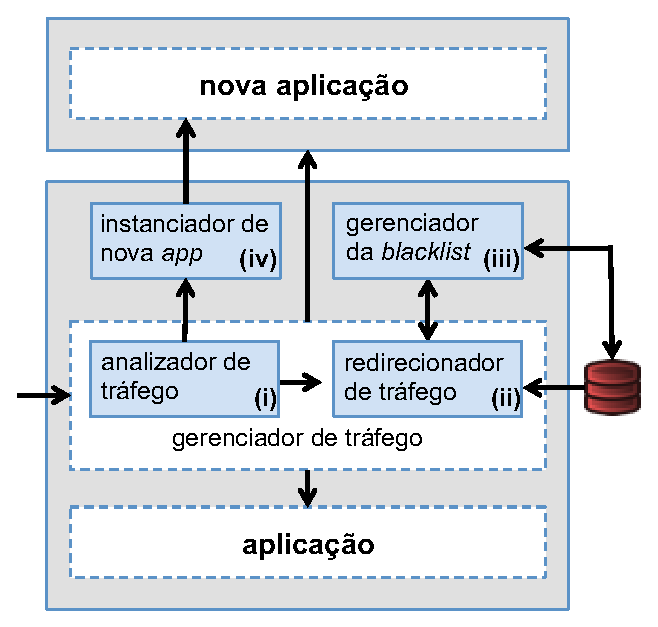
\includegraphics[width=0.55\textwidth]{arq.eps}
\caption{Ilustração da proposta de arquitetura para mitigação de ataques DDoS}
\label{fig:arq}
\end{figure}



O sub módulo AT observa o comportamento do tráfego de entrada para a aplicação de forma pró-ativa. Focando-se na estimativa de quantidade de tráfego e de processamento no servidor, este sub módulo realiza medição para verificar a existência de um possível ataque DDoS. Caso detectado, o sub módulo INA é ativado. O INA criará uma nova instância da aplicação em outro servidor na \emph{cloud}, consequentemente com um endereço IP diferente. Com isso, o sub módulo RT passará a tratar todo o tráfego de entrada, respondendo com um redirecionamento para a nova instância da aplicação. Parte-se do princípio que atacantes DDoS não interpretam as respostas obtidas do servidor, pois se interpretarem, sua eficiência é reduzida. Desta maneira, apenas os clientes legítimos serão, de fato, redirecionado à nova aplicação.

Ao redirecionar algum cliente para a nova instância, o endereço deste cliente, seja ele legítimo ou não, será adicionado em uma \emph{blacklist}. Os clientes presentes nesta lista terão suas requisições descartadas, a fim de reduzir o custo de processamento de respostas no servidor. Entretanto, como o cliente legítimo foi informado antes de seu endereço entrar nesta \emph{blacklist}, isso não será um problema, pois ele já terá acesso à nova instância. Serão empregadas entradas com tempo de validade nesta \emph{blacklist}, dado que respostas podem ser perdidas. O tempo de validade na lista aumentará exponencialmente, para diminuir ainda mais a sobrecarga. Cabem ao GB este papel de adicionar endereços e gerenciar sua saída e o tempo de validade que aumenta exponencialmente.

%Tal procedimento é adotado baseando-se no princípio de que o atacante não afetará a nova instância da aplicação, pois ele não interpretará as respostas que informam o IP da nova instância e continuará enviando solicitações em direção ao endereço antigo da aplicação.




Focamos na estimativa de quantidade de tráfego para direcionar o tráfego pelo módulo 


Falar sobre:
Banco de dados Redis, chave, valor....
Blacklist com TTL para reenvio de novo endereco da aplicacao, para onde ela foi movida, verificar a questao de performance...
Arquitetura......




% \newpage
% \bibliographystyle{unsrt}
\bibliographystyle{sbc}
\bibliography{proposta3}
\end{document}
